\chapter{Strumenti di front-end}

% Alcuni output (Vite, Sass) contengono caratteri che listings, con LuaLaTeX,
% stamperebbe fuori posto, in fondo alla riga precedente. Nel sorgente sono
% scritti con segnaposto latin-1 che \wtglifi sostituisce al momento della
% composizione: ¤ e' la freccia di Vite (che nessun font della dispensa
% contiene: la si disegna), ¢ la spunta, ¦ la barra verticale, ¯ la lineetta,
% ¸ e ¹ gli estremi della cornice dei messaggi di Sass, ¬ il trattino
% tipografico (come nel capitolo 19).
\newcommand{\wtfrecciaterm}{\tikz[baseline=-0.6ex]{\draw[line width=1.3pt,
  -{Stealth[length=3.4pt,width=5pt]}, draw=consolefg] (0,0) -- (0.52em,0);}}
\newcommand{\wtglifi}{\lstset{extendedchars=true,
  literate={¤}{{\wtfrecciaterm}}1 {¢}{{✓}}1 {¦}{{│}}1 {¯}{{—}}1
           {¸}{{╷}}1 {¹}{{╵}}1 {¬}{{\textendash}}1}}

Abbiamo iniziato dalle tecnologie fondamentali (HTML, CSS, JavaScript),
costruito pagine statiche e poi siamo passati alla programmazione lato server.
Le pagine che generavamo dinamicamente restavano però semplici: un solo foglio
di stile, pochissimo JavaScript lato client, nessuna libreria esterna.

I front-end moderni sono molto più complessi:

\begin{itemize}
  \item il codice JavaScript lato client è sempre più articolato: si usano molte
        librerie e moduli, si transpila e si applica il \textit{downleveling}
        (capitolo 19), si ottimizzano i file serviti;
  \item per i fogli di stile si usano spesso pre- e post-processori, come Sass.
\end{itemize}

Servono strumenti che assistano lo sviluppatore e automatizzino questi
passaggi. In questo capitolo vediamo i principali: i \textbf{pre- e
post-processori CSS} (in particolare \term{Sass}), i \textbf{framework CSS}, il
\textbf{bundling} e la \textbf{minificazione}, e infine \term{Vite}, che riunisce
in un solo strumento il server di sviluppo e la build.

\info{Le versioni di questo capitolo}{
  Tutti gli esempi sono stati eseguiti davvero, con Node.js 22.22.0 e npm 10.9.4:
  Sass 1.108.2, PostCSS 8.5.33 (con \code{postcss-preset-env} 11.6.3 e
  Autoprefixer 10.7.0), Bootstrap 5.3.9, Terser 5.51.3, esbuild 0.28.2,
  \code{create-vite} 9.3.4, Vite 8.3.8 e TypeScript 7.0.2. Gli output riportati
  sono quelli reali; i percorsi sono abbreviati in
  \codel{[cartella del progetto]} e le parti tralasciate segnate con
  \code{...}. Le slide mostrano Vite 6 e 8 e TypeScript 6: dove il risultato
  cambia, lo diciamo.}

\section{Pre- e post-processori CSS}

Il CSS di per sé può essere piacevole, ma i fogli di stile diventano presto
grandi, complessi e difficili da mantenere. Gli strumenti di pre- e
post-elaborazione permettono di creare in modo efficiente fogli di stile
robusti, scalabili e ottimizzati.

\begin{figure}[H]
  \centering
  \begin{tikzpicture}[font=\Lato\small,
      n/.style={wtnode, minimum width=2.9cm, minimum height=1.0cm},
      f/.style={wtnodeplain, minimum width=2.2cm, minimum height=0.9cm},
      a/.style={-{Stealth[length=5pt,width=4pt]}, line width=0.85pt,
                draw=neutral!45!black}]

    \node[f] (src) at (0,0) {file sorgente};
    \node[n, draw=orange-gradient-6, fill=orange-gradient-1!40!white]
      (pre) at (3.4,0) {\textbf{Pre-processore}};
    \node[f] (c1) at (6.5,0) {CSS};
    \node[n, draw=azure-gradient-6, fill=azure-gradient-1!45!white]
      (post) at (9.6,0) {\textbf{Post-processore}};
    \node[f] (c2) at (12.6,0) {CSS};

    \draw[a] (src) -- (pre);
    \draw[a] (pre) -- (c1);
    \draw[a] (c1) -- (post);
    \draw[a] (c2.south) -- ++(0,-0.9) node[below, font=\Lato\scriptsize,
                                          text=neutral!30!black] {browser};
    \draw[a] (post) -- (c2);
  \end{tikzpicture}
  \caption{La catena di elaborazione di un foglio di stile moderno.}
  \label{fig:css-pipeline}
\end{figure}

\subsection{Pre-processori}

I \term{pre-processori CSS} sono \guillemotleft compilatori\guillemotright\
speciali che generano codice CSS a partire da file scritti in una sintassi
propria. Tale sintassi si può vedere come un'\textbf{estensione} del CSS di
base, che introduce funzionalità nuove (per esempio le variabili) per scrivere
fogli di stile manutenibili in modo più efficiente. I più diffusi sono
\term{Sass}, \term{LESS} e \term{Stylus}.

\subsection{Post-processori}

I \term{post-processori} elaborano e trasformano automaticamente fogli di stile
già esistenti. Si usano tipicamente per:

\begin{itemize}
  \item il \textbf{downleveling}, cioè riscrivere costrutti recenti in forme
        comprese anche dai browser più vecchi (\urlx{https://preset-env.cssdb.org/});
  \item l'\textbf{autoprefissatura}, cioè aggiungere i prefissi specifici dei
        browser (\urlx{https://autoprefixer.github.io/});
  \item le \textbf{ottimizzazioni}, come la minificazione o l'eliminazione delle
        parti inutilizzate;
  \item l'\textbf{imposizione di convenzioni} e il rilevamento di errori.
\end{itemize}

Il post-processore più diffuso è \term{PostCSS}: di per sé non fa quasi nulla,
ma esegue dei \textit{plugin}, ognuno con il suo compito. Lo installiamo nel
progetto insieme alla sua interfaccia a riga di comando e ai due plugin che
realizzano gli esempi delle slide:

\begin{console}[Terminale]
$ npm install -D postcss postcss-cli postcss-preset-env autoprefixer

added 135 packages, and audited 136 packages in 3s

109 packages are looking for funding
  run `npm fund` for details

found 0 vulnerabilities
\end{console}

Il primo esempio è il \textbf{downleveling} di un colore espresso con
\code{oklch()}, una notazione recente che descrive un colore con luminosità,
croma e tinta. Il plugin
\code{postcss-preset-env} lo converte in \code{rgb()} (l'opzione
\code{-{}-no-map} evita di accodare al risultato la \textit{source map}, di cui
parleremo con Sass):

\begin{affianco}[0.42]
\begin{lstlisting}[style=css, name=oklch.css]
body {
  color: oklch(61% 0.2 29);
}
\end{lstlisting}
\risultato
\begin{console}[Terminale]
$ npx postcss oklch.css --use postcss-preset-env --no-map
body {
  color: rgb(226, 65, 52);
}
\end{console}
\end{affianco}

Nella slide il risultato è \code{rgb(225, 65, 52)}: una differenza di
arrotondamento fra le versioni del plugin, invisibile a occhio.

Il secondo esempio è l'\textbf{autoprefissatura}, affidata al plugin
\term{Autoprefixer}. Proviamolo sulla transizione delle slide:

\begin{affianco}[0.42]
\begin{lstlisting}[style=css, name=transition.css]
.example {
  transition: all .5s;
}
\end{lstlisting}
\risultato
\begin{console}[Terminale]
$ npx postcss transition.css --use autoprefixer --no-map
.example {
  transition: all .5s;
}
\end{console}
\end{affianco}

Nessun prefisso: Autoprefixer aggiunge solo quelli che servono ai browser da
supportare, e la proprietà \code{transition} senza prefisso funziona ovunque da
anni. Quali siano i browser da supportare lo decide \term{Browserslist}, una
lista condivisa da molti strumenti (Autoprefixer, \code{postcss-preset-env},
Babel, Vite\ldots). Senza indicazioni vale la query \code{defaults}:

\begin{console}[Terminale]
$ npx browserslist --coverage
These browsers account for 85.68% of all users globally
\end{console}

Se però dobbiamo supportare browser molto vecchi, per esempio Safari 6 e
Opera 12 (del 2012), i prefissi compaiono, esattamente come nella slide. La
variabile d'ambiente \code{BROWSERSLIST} sostituisce la lista predefinita:

\begin{console}[Terminale]
$ BROWSERSLIST='Safari 6, Opera 12' npx postcss transition.css --use autoprefixer --no-map
.example {
  -webkit-transition: all .5s;
  -o-transition: all .5s;
  transition: all .5s;
}
\end{console}

In un progetto vero la lista si scrive una volta per tutte nel
\code{package.json} (chiave \code{"browserslist"}) o in un file
\code{.browserslistrc}, e tutti gli strumenti la leggono da lì.

\subsection{Quanto sono usati}

Il sondaggio \textit{State of CSS} 2023 chiedeva quali pre- o post-processori si
usassero abitualmente. Sass è il più diffuso, seguito da PostCSS (i dati sono
quelli riportati nelle slide):

\begin{figure}[H]
  \centering
  \begin{tikzpicture}[font=\Lato\footnotesize]
    % 1 cm = 500 risposte (lunghezze calcolate a mano: 4746/500 = 9,49...)
    \foreach \y/\nome/\n/\l/\col in {
        0/Sass\slash SCSS/4746/9.49/primary,
        -0.62/PostCSS/3022/6.04/primary,
        -1.24/Nessuna risposta/2571/5.14/neutral,
        -1.86/Nessuno/992/1.98/neutral,
        -2.48/Less/941/1.88/primary,
        -3.10/Stylus/291/0.58/primary,
        -3.72/Assembler CSS/18/0.04/primary} {
      \node[anchor=east, text=neutral!20!black] at (-0.15,\y) {\nome};
      \fill[\col!55!white] (0,\y-0.2) rectangle (\l,\y+0.2);
      \node[anchor=west, font=\Lato\scriptsize, text=neutral!25!black]
        at (\l,\y) {\n};
    }
    \draw[neutral!50!white, line width=0.5pt] (0,0.35) -- (0,-4.07);
  \end{tikzpicture}
  \caption{Pre- e post-processori usati abitualmente (State of CSS 2023,
           6599 risposte alla domanda).}
  \label{fig:state-of-css}
\end{figure}

\section{Sass}

\term{Sass} si autodefinisce \guillemotleft CSS con i superpoteri\guillemotright\
ed è attualmente il pre-processore CSS più diffuso. Esiste dal 2006, cioè da
vent'anni. Gli altri pre-processori offrono grosso modo le stesse funzionalità
con una sintassi leggermente diversa.

\subsection{Installazione}

Le opzioni di installazione sono descritte sul sito ufficiale; la più semplice
è installare Sass con npm, globalmente, così che il comando \code{sass} sia
disponibile nel percorso di sistema:

\begin{console}[Terminale]
$ npm install -g sass

added 12 packages in 2s

5 packages are looking for funding
  run `npm fund` for details
$ sass --version
1.108.2 compiled with dart2js 3.13.7
$ sass --help | head -n 4
Compile Sass to CSS.

Usage: sass <input.scss> [output.css]
       sass <input.scss>:<output.css> <input/>:<output/> <dir/>
\end{console}

La versione rivela un dettaglio: Sass è scritto in Dart (è \term{Dart Sass},
l'implementazione di riferimento), e il pacchetto npm ne contiene una versione
compilata in JavaScript. In un progetto lo si installa più spesso come
dipendenza di sviluppo, con \code{npm install -D sass}, come faremo con Vite.

\subsection{Due sintassi}

Sass supporta due sintassi diverse:

\begin{center}
\renewcommand{\arraystretch}{1.4}
\begin{tabular}{@{}>{\raggedright\arraybackslash}p{6.3cm}@{\hspace{1.0cm}}>{\raggedright\arraybackslash}p{6.3cm}@{}}
  \textbf{Sintassi SCSS} & \textbf{Sintassi indentata} \\
  Estensione \code{.scss}. & Estensione \code{.sass}. \\
  È un \textbf{superset} del CSS: qualunque CSS valido è SCSS valido.
  & Basata sull'indentazione, come Python. \\
  È la sintassi più diffusa. & Era la sintassi originale. \\
\end{tabular}
\end{center}

Lo stesso foglio di stile nelle due sintassi, così come compare nelle slide,
produce lo stesso CSS (senza un file di destinazione, \code{sass} stampa il
risultato nel terminale):

\begin{affianco}[0.5]
\begin{lstlisting}[style=css, name=stile.scss]
$font-stack: Helvetica, sans-serif;
$primary-color: #333;

body {
  font: 100% $font-stack;
  color: $primary-color;
}
\end{lstlisting}
\begin{lstlisting}[style=css, name=stile.sass]
$font-stack: Helvetica, sans-serif
$primary-color: #333

body
  font: 100% $font-stack;
  color: $primary-color;
\end{lstlisting}
\risultato
\begin{console}[Terminale]
$ sass stile.scss
body {
  font: 100% Helvetica, sans-serif;
  color: #333;
}
$ sass stile.sass
body {
  font: 100% Helvetica, sans-serif;
  color: #333;
}
\end{console}
\end{affianco}

Nella versione indentata delle slide le dichiarazioni dentro \code{body}
terminano con il punto e virgola, che in quella sintassi non serve. Le versioni
recenti di Sass lo tollerano (dalla 1.84); le precedenti si rifiutavano di
compilare:

{\wtglifi
\begin{console}[Terminale]
$ npx -y sass@1.83.0 stile.sass
Error: semicolons aren't allowed in the indented syntax.
  ¸
5 ¦   font: 100% $font-stack;
  ¦                         ^
  ¹
  stile.sass 5:25  root stylesheet
\end{console}
}

Senza punti e virgola il file funziona con tutte le versioni. Nel resto del
capitolo useremo la sintassi SCSS.

\subsection{Variabili}

Sass supporta le \term{variabili}: permettono di riusare valori in tutto il
foglio di stile e, al momento della compilazione, vengono sostituite dal loro
valore. Compiliamo il file delle slide come fa la slide, indicando anche il file
di destinazione:

\begin{affianco}[0.42]
\begin{lstlisting}[style=css, name=file.scss]
$font-stack: Helvetica, sans-serif;
$primary-color: #333;

body {
  font: $font-stack;
  color: $primary-color;
}
\end{lstlisting}
\risultato
\begin{console}[Terminale]
$ sass file.scss file.css
$ ls
file.css
file.css.map
file.scss
$ cat file.css
body {
  font: Helvetica, sans-serif;
  color: #333;
}

/*# sourceMappingURL=file.css.map */
\end{console}
\end{affianco}

Oltre a \code{file.css}, Sass ha scritto \code{file.css.map}, una
\term{source map}, e l'ha collegata al CSS con il commento finale:

\begin{console}[Terminale]
$ cat file.css.map
{"version":3,"sourceRoot":"","sources":["file.scss"],"names":[],"mappings":"AAGA;EACE,MAJW;EAKX,OAJc","file":"file.css"}
\end{console}

Il campo \code{mappings} codifica, in forma compatta, da quale riga e colonna di
\code{file.scss} viene ogni pezzo di \code{file.css}. Gli strumenti per
sviluppatori del browser la usano per mostrare, accanto a una regola, il file
Sass e la riga in cui l'abbiamo scritta, anziché il CSS generato. Con
\code{-{}-no-source-map} la mappa non viene prodotta.

\begin{warningbox}{{Una dichiarazione che il browser scarta}}
  Il CSS generato dalla slide contiene \code{font: Helvetica, sans-serif}, che
  \textbf{non è valido}: la proprietà abbreviata \code{font} richiede almeno la
  dimensione e la famiglia (la slide sulle due sintassi infatti scrive
  \code{font: 100\% \$font-stack}). Sass non controlla il significato delle
  proprietà e lo copia così com'è; il browser lo scarta. Lo verifichiamo con
  Chromium, guidato da Playwright: per ogni paragrafo lo script stampa che cosa
  resta della regola e la famiglia di caratteri effettivamente usata.

  \begin{console}[Terminale]
$ node font.js
.senza-dimensione: {  } -> font-family "Times New Roman"
.con-dimensione: { font: 100% Helvetica, sans-serif; } -> font-family Helvetica, sans-serif
\end{console}

  La prima regola è rimasta vuota, e il testo usa il carattere predefinito. In
  alternativa si può scrivere \codel{font-family: \$font-stack}.
\end{warningbox}

\subsection{Annidamento}

In HTML esiste una chiara gerarchia di elementi annidati; nel CSS tradizionale
le regole non si possono annidare. Sass introduce l'\term{annidamento}, che può
rendere il codice più leggibile. Ecco l'esempio delle slide:

\begin{affianco}[0.55]
\begin{lstlisting}[style=css, name=elem.scss, morecomment={[l]{//}}]
.elem {
  color: red;
  span {
    color: blue;
    a {
      color: green; //applies to <a>s contained in <span>s contained in .elem
    }
  }
}
\end{lstlisting}
\risultato
\begin{console}[Terminale]
$ sass elem.scss
.elem {
  color: red;
}
.elem span {
  color: blue;
}
.elem span a {
  color: green;
}
\end{console}
\end{affianco}

Ogni regola annidata diventa una regola con il selettore discendente completo.
Il commento con \code{//} è un \textit{commento silenzioso}: resta nel sorgente
ma non arriva nel CSS (i commenti \code{/* */} invece vengono copiati). Il
secondo esempio costruisce lo stile di una barra di navigazione:

\begin{affianco}[0.42]
\begin{lstlisting}[style=css, name=nesting.scss]
nav {
  ul {
    margin: 0;
    padding: 0;
    list-style: none;
  }

  li { display: inline-block; }

  a {
    display: block;
    padding: 6px 12px;
    text-decoration: none;
  }
}
\end{lstlisting}
\risultato
\begin{console}[Terminale]
$ sass nesting.scss
nav ul {
  margin: 0;
  padding: 0;
  list-style: none;
}
nav li {
  display: inline-block;
}
nav a {
  display: block;
  padding: 6px 12px;
  text-decoration: none;
}
\end{console}
\end{affianco}

\warning{Annidare troppo è una cattiva pratica}{
  Ogni livello di annidamento aggiunge un elemento al selettore generato, e
  quindi aumenta la \textbf{specificità}. Selettori troppo specifici sono
  difficili da sovrascrivere e rendono il foglio di stile fragile: torna qui
  tutto quello che abbiamo studiato sulla cascata nel capitolo 3. Come regola
  pratica, non superare i tre livelli.}

\info{L'annidamento è arrivato anche nel CSS}{
  Dal 2023 i browser supportano l'annidamento \textbf{nativo}, con il selettore
  \code{\&} (capitolo 14): il foglio di stile del progetto di esempio di Vite,
  più avanti, lo usa già. Sass resta utile per tutto il resto (variabili
  risolte alla compilazione, mixin, moduli, cicli), e il CSS annidato che
  produce funziona anche nei browser che l'annidamento non lo conoscono.}

\subsection{Mixin}

I \term{mixin} permettono di riusare un gruppo di dichiarazioni CSS o Sass. Si
dichiarano con la regola \code{@mixin} seguita da un identificatore e si
includono con \code{@include}:

\begin{affianco}[0.45]
\begin{lstlisting}[style=css, name=mixins.scss]
@mixin clear-list {
  list-style-type: none;
  padding: 0; margin: 0;
  li {
    display: inline-block;
  }
}

nav ul {
  background-color: aliceblue;
  @include clear-list;
}
\end{lstlisting}
\risultato
\begin{console}[Terminale]
$ sass mixins.scss
nav ul {
  background-color: aliceblue;
  list-style-type: none;
  padding: 0;
  margin: 0;
}
nav ul li {
  display: inline-block;
}
\end{console}
\begin{browser}[nav]
  \colorbox{css-aliceblue}{\makebox[\dimexpr\linewidth-2\fboxsep][l]{Home\quad Corsi\quad Contatti}}
\end{browser}
\end{affianco}

Le dichiarazioni del mixin vengono copiate dove lo si include, e anche la regola
annidata per \code{li} segue il selettore di chi lo include. I mixin possono
anche avere \textbf{parametri}, con valori predefiniti:

\begin{affianco}[0.45]
\begin{lstlisting}[style=css, name=theme.scss]
@mixin theme($color: DarkBlue) {
  background: $color;
  color: #fff;
}

.info {
  @include theme;
}

.danger {
  @include theme($color: DarkRed);
}
\end{lstlisting}
\risultato
\begin{console}[Terminale]
$ sass theme.scss
.info {
  background: DarkBlue;
  color: #fff;
}

.danger {
  background: DarkRed;
  color: #fff;
}
\end{console}
\begin{browser}[theme]
  \colorbox{css-darkblue}{\makebox[\dimexpr\linewidth-2\fboxsep][l]{\color{white}.info}}\\[3pt]
  \colorbox{css-darkred}{\makebox[\dimexpr\linewidth-2\fboxsep][l]{\color{white}.danger}}
\end{browser}
\end{affianco}

\subsection{Moduli e parziali}

Un foglio di stile Sass può usarne un altro come \term{modulo}, con la regola
\code{@use}: le variabili del modulo si leggono con il prefisso del suo nome, e
il CSS generato contiene anche le regole del modulo.

\begin{affianco}[0.45]
\begin{lstlisting}[style=css, name=base.scss]
$font-stack: Helvetica, sans-serif;
$primary-color: #333;

body {
  font: $font-stack;
  color: $primary-color;
}
\end{lstlisting}
\begin{lstlisting}[style=css, name=example.scss]
@use 'base';

.inverse {
  background: base.$primary-color;
  color: white;
}
\end{lstlisting}
\risultato
\begin{console}[Terminale]
$ sass example.scss
body {
  font: Helvetica, sans-serif;
  color: #333;
}

.inverse {
  background: #333;
  color: white;
}
\end{console}
\end{affianco}

Nella slide la seconda regola generata è scritta \code{background-color: \#333},
ma Sass non cambia il nome della proprietà: scrive \code{background}, come nel
sorgente. Torna anche il \code{font} non valido del paragrafo sulle variabili.

I file Sass il cui nome inizia con un trattino basso sono detti
\term{parziali}: sono pensati solo per essere inclusi da altri file, e Sass non
genera per essi un file CSS autonomo. Un file che raccoglie tutte le variabili
è un buon esempio di parziale. Compilando un'intera cartella
(\code{sass scss:css}, cioè \guillemotleft da \code{scss} a
\code{css}\guillemotright) lo si vede bene:

\begin{affianco}[0.45]
\begin{lstlisting}[style=css, name=scss/_variables.scss]
$primary-color: purple;
$accent-color: orange;
$background-color: beige;
\end{lstlisting}
\begin{lstlisting}[style=css, name=scss/style.scss]
@use 'variables';

body {
  color: variables.$primary-color;
  background-color: variables.$background-color;
}

a {
  color: variables.$accent-color;
}
\end{lstlisting}
\risultato
\begin{console}[Terminale]
$ sass scss:css
$ ls scss css
css:
style.css
style.css.map

scss:
_variables.scss
style.scss
$ cat css/style.css
body {
  color: purple;
  background-color: beige;
}

a {
  color: orange;
}

/*# sourceMappingURL=style.css.map */
\end{console}
\end{affianco}

Nella cartella \code{css} c'è solo \code{style.css}: il parziale è stato usato,
ma non compilato da solo. Nella regola \code{@use} il trattino basso e
l'estensione si omettono.

\subsection{Liste e mappe}

Le \term{liste} sono sequenze di valori separati da virgole, spazi o barre
(purché il separatore sia lo stesso in tutta la lista). Le \term{mappe} sono
sequenze di coppie chiave-valore, nella forma \code{<chiave>: <valore>}, con
chiavi uniche. I moduli predefiniti \code{sass:list} e \code{sass:map} offrono
le funzioni per leggerle:

\begin{affianco}[0.55]
\begin{lstlisting}[style=css, name=liste.scss]
@use "sass:list";
@use "sass:map";

$list: (120px, 240px, 480px, 800px);
$map: ("xs": 480px, "md": 768px, "lg": 1024px);

.terzo { width: list.nth($list, 3); }
.medio { max-width: map.get($map, "md"); }
\end{lstlisting}
\risultato
\begin{console}[Terminale]
$ sass liste.scss
.terzo {
  width: 480px;
}

.medio {
  max-width: 768px;
}
\end{console}
\end{affianco}

Gli elementi di una lista si contano da 1, non da 0: il terzo è
\code{480px}.

\subsection{Regole di controllo del flusso}

Sass offre regole per decidere \textbf{se} emettere degli stili, o per emetterli
più volte con piccole variazioni: si può pensarlo come un motore di template
(capitolo 12) per generare CSS. \code{@if}/\code{@else} emettono stili in modo
condizionale, \code{@each} itera sugli elementi di una lista o di una mappa,
\code{@for} e \code{@while} hanno il significato consueto.

\begin{affianco}[0.55]
\begin{lstlisting}[style=css, name=avatar.scss]
@use "sass:math";

@mixin avatar($size, $circle: false) {
  width: $size;
  height: $size;

  @if $circle {
    border-radius: math.div($size, 2);
  }
}

.square-av {
  @include avatar(100px, $circle: false);
}
.circle-av {
  @include avatar(100px, $circle: true);
}
\end{lstlisting}
\risultato
\begin{console}[Terminale]
$ sass avatar.scss
.square-av {
  width: 100px;
  height: 100px;
}

.circle-av {
  width: 100px;
  height: 100px;
  border-radius: 50px;
}
\end{console}
\begin{browser}[avatar]
  \tikz{\fill[primary!35!white] (0,0) rectangle (1.2,1.2);
        \fill[primary!35!white] (2.2,0.6) circle (0.6);}
\end{browser}
\end{affianco}

La divisione si scrive con \code{math.div()}, dal modulo \code{sass:math}: in
Sass la barra \code{/} è anche un separatore (si pensi a
\code{font: 16px/1.5}), e come operatore di divisione è deprecata.

\code{@each} percorre una mappa prendendo a ogni giro la chiave e il valore. Con
l'interpolazione \code{\#\{\ldots\}} il valore di una variabile finisce dentro un
selettore:

\begin{affianco}[0.52]
\begin{lstlisting}[style=css, name=hidden.scss]
$sizes: ("xs": 480px, "md": 768px, "lg": 1024px);

@each $sizeName, $sizeMaxWidth in $sizes {
  @media screen and (max-width: $sizeMaxWidth) {
    .hidden-#{$sizeName} {
      display: none;
    }
  }
}
\end{lstlisting}
\risultato
\begin{console}[Terminale]
$ sass hidden.scss
@media screen and (max-width: 480px) {
  .hidden-xs {
    display: none;
  }
}
@media screen and (max-width: 768px) {
  .hidden-md {
    display: none;
  }
}
@media screen and (max-width: 1024px) {
  .hidden-lg {
    display: none;
  }
}
\end{console}
\end{affianco}

Da tre righe di dichiarazione si generano tre media query complete (la slide
omette la terza per brevità): è esattamente il tipo di ripetizione che rende
ingestibili i fogli di stile scritti a mano. Le slide nominano \code{@for} senza
un esempio; eccone uno, con un ciclo che genera tre classi di margine:

\begin{affianco}[0.52]
\begin{lstlisting}[style=css, name=margini.scss]
@for $i from 1 through 3 {
  .mt-#{$i} {
    margin-top: $i * 0.25rem;
  }
}
\end{lstlisting}
\risultato
\begin{console}[Terminale]
$ sass margini.scss
.mt-1 {
  margin-top: 0.25rem;
}

.mt-2 {
  margin-top: 0.5rem;
}

.mt-3 {
  margin-top: 0.75rem;
}
\end{console}
\end{affianco}

Sass fa i conti con le unità di misura: \code{3 * 0.25rem} è \code{0.75rem}.
È così che i framework CSS generano intere famiglie di classi di utilità, come
vedremo ora.

\section{Framework CSS}

Anche scrivendo il CSS del front-end ci si ritrova a risolvere sempre gli stessi
problemi: creare un sistema di impaginazione, definire una tipografia coerente,
dare stile a tabelle, liste e componenti dell'interfaccia, azzerare gli stili
predefiniti dei browser (gli stili dello \textit{user agent}) per ottenere un
aspetto uniforme ovunque. Per fortuna non serve ripartire da zero ogni volta.

Esistono molti \term{framework CSS} che forniscono un insieme di stili di uso
generale, utilizzabili così come sono oppure come base da rifinire. Fra i più
diffusi: \term{Bootstrap} (il più popolare, nato in Twitter),
\term{Tailwind} (noto per l'approccio \textit{utility-first}: al posto di
componenti già pronti offre migliaia di piccole classi, una per proprietà),
\term{Materialize}, \term{Foundation}, \term{Bulma}, \term{PureCSS}.

\info{Non sono framework in senso stretto}{
  Nonostante il nome, non sono framework come quelli visti nel capitolo 15: non
  c'è inversione del controllo, non chiamano il nostro codice. Sono
  \textbf{insiemi di fogli di stile} da importare, con classi da applicare agli
  elementi.}

Un framework è uno o più file CSS: basta importarli nelle nostre pagine e usare
le classi che forniscono, come descritto nella documentazione. I file si possono
scaricare e servire dal proprio server, oppure si può ricorrere a una
\term{CDN} (\textit{Content Delivery Network}) che li ospita per noi: comodo per
prototipare, ma con qualche implicazione sulla privacy, dato che ogni visitatore
contatta un server di terze parti.

\subsection{Un esempio con Bootstrap}

Riproduciamo la pagina dimostrativa delle slide, costruita con Bootstrap 5.3.
Installiamo il framework con npm, che lo scarica in \code{node\_modules}:

\begin{console}[Terminale]
$ npm install bootstrap

added 2 packages, and audited 3 packages in 576ms

2 packages are looking for funding
  run `npm fund` for details

found 0 vulnerabilities
$ npm ls
bootstrap@1.0.0 [cartella del progetto]
`-- bootstrap@5.3.9
\end{console}

Il pacchetto contiene il CSS già compilato, in \code{dist/css} (in versione
normale e minificata), e i sorgenti Sass, in \code{scss}. La pagina importa il
CSS minificato e usa le classi di Bootstrap: \code{container} per il contenitore
centrato, \code{row} e \code{col} per la griglia, \code{card} per i riquadri,
\code{btn} con le sue varianti per i pulsanti, \code{table} per la tabella.

\begin{lstlisting}[style=html, name=index.html, firstnumber=3]
<head>
  <meta charset="utf-8">
  <meta name="viewport" content="width=device-width, initial-scale=1">
  <title>Pricing</title>
  <link rel="stylesheet" href="node_modules/bootstrap/dist/css/bootstrap.min.css">
</head>
\end{lstlisting}

\begin{lstlisting}[style=html, name=index.html, firstnumber=37]
      <div class="col">
        <div class="card h-100 border-secondary">
          <div class="card-header text-bg-secondary">Pro</div>
          <div class="card-body">
            <h2 class="card-title">$15<small class="text-body-secondary">/mo</small></h2>
            <p>20 hello world examples included</p>
            <button class="btn btn-secondary w-100">Get started</button>
          </div>
        </div>
      </div>
\end{lstlisting}

Gli altri due riquadri sono uguali, con \code{btn-outline-primary} e
\code{btn-primary}. Ecco la pagina in Chromium:

\begin{browser}[index.html]
  \centering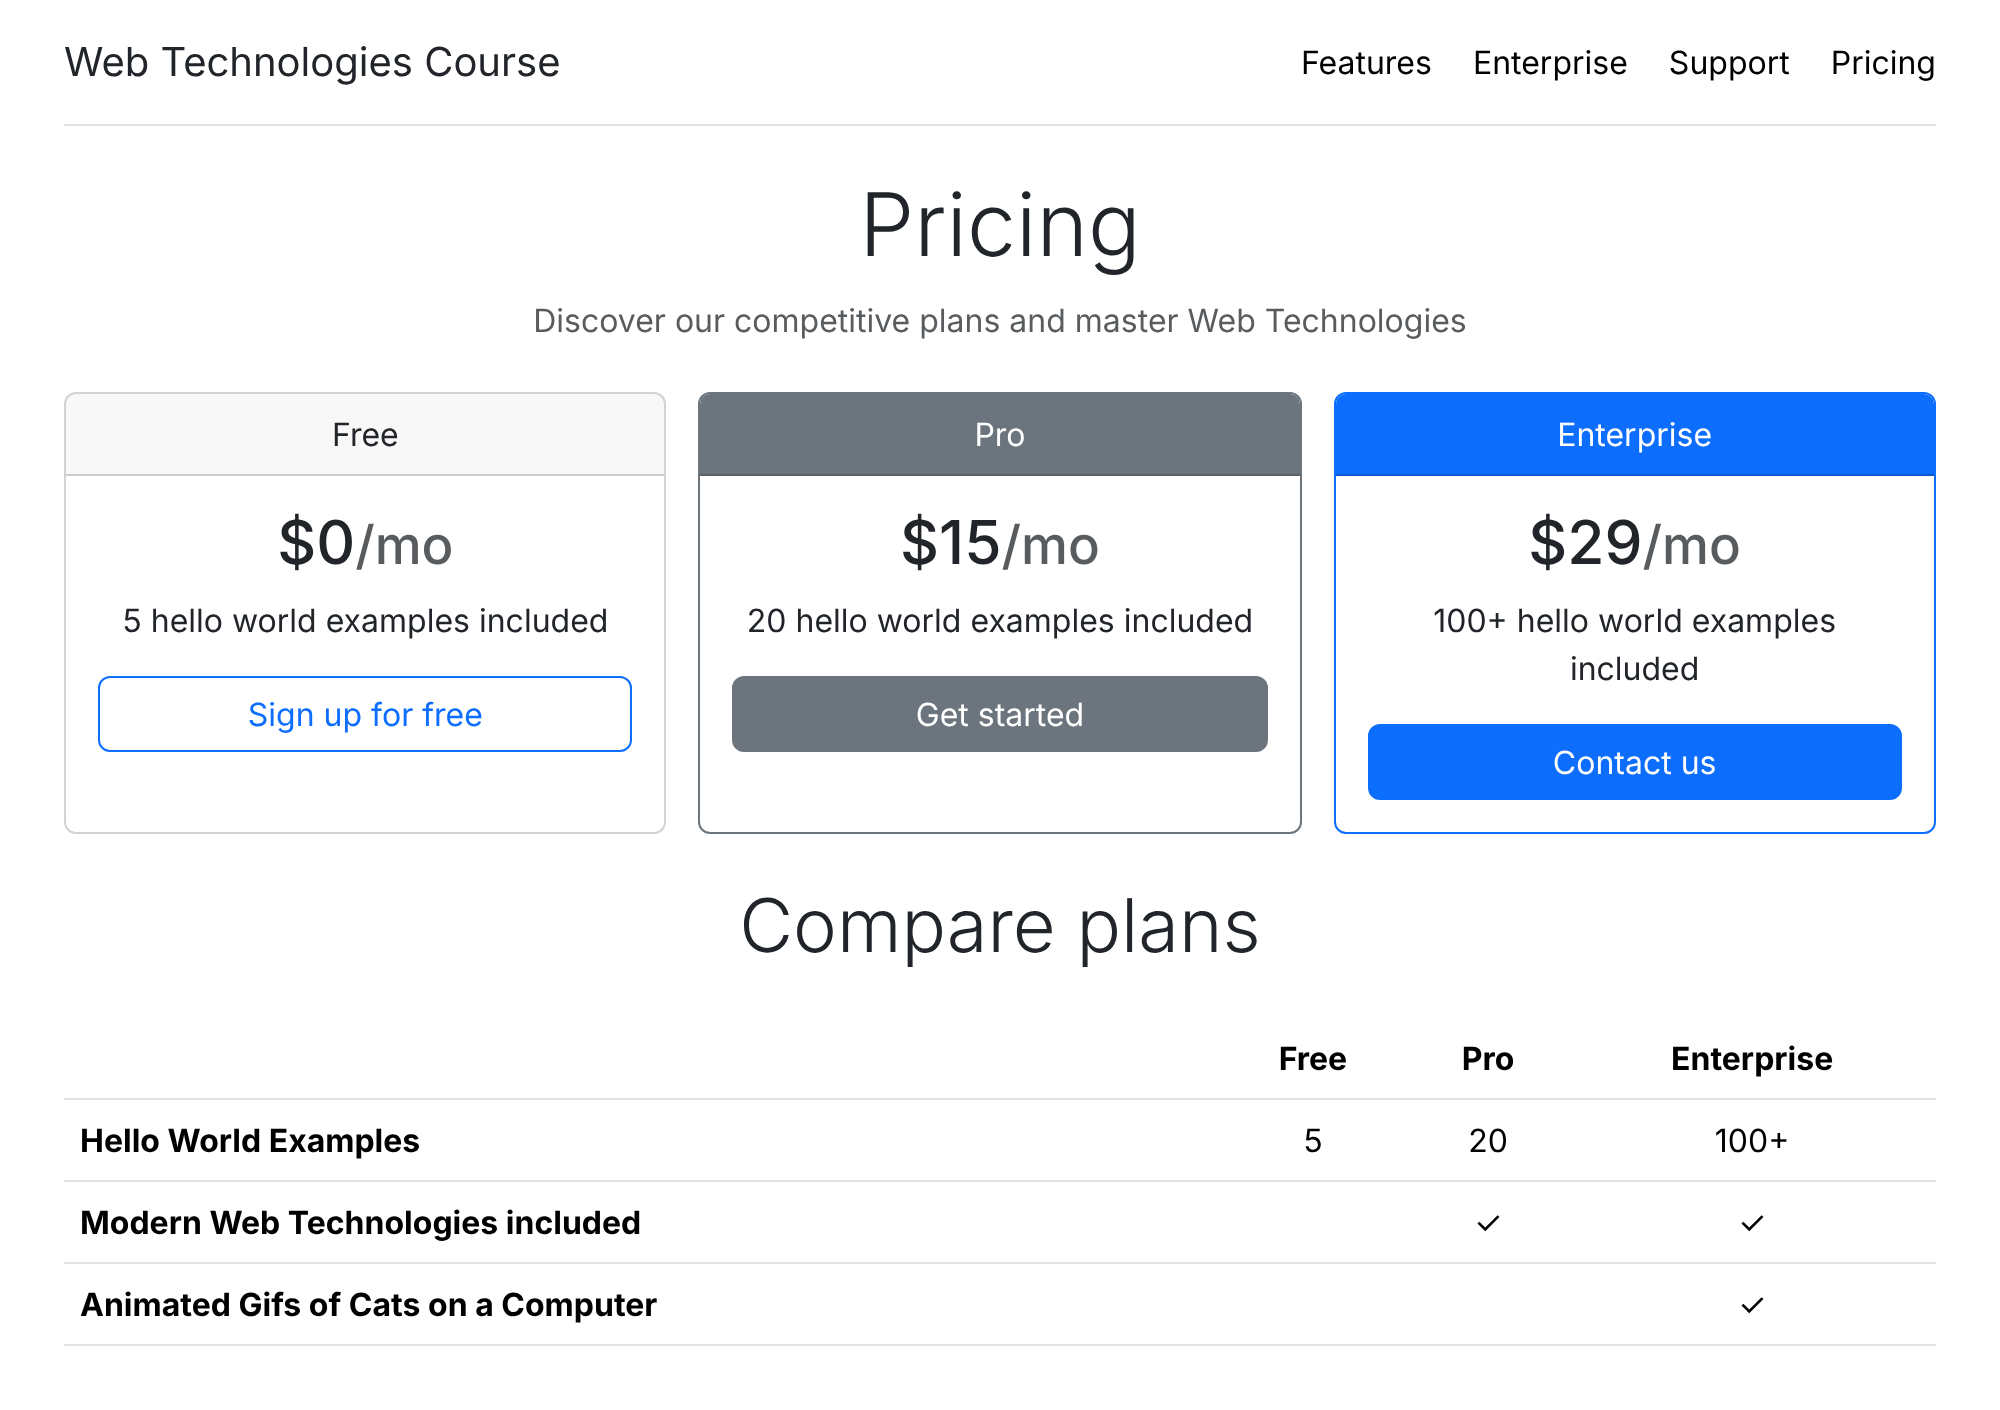
\includegraphics[width=0.92\linewidth]{sources/frontend-bootstrap.png}
\end{browser}

Non abbiamo scritto una riga di CSS: margini, tipografia, colori, bordi e
griglia vengono tutti da Bootstrap.

\subsection{Personalizzare un framework}

Potremmo però non volere che il nostro sito assomigli a tutti gli altri
costruiti con lo stesso framework, e gli stili predefiniti potrebbero non
soddisfare qualche esigenza particolare. Le strade sono due:

\begin{itemize}
  \item la maggior parte dei framework CSS è costruita con Sass o strumenti
        simili: si possono \textbf{cambiare le variabili} di build (colori,
        caratteri, dimensioni) e ricompilare il framework;
  \item si possono definire stili personalizzati che \textbf{sovrascrivono}
        alcuni stili del framework.
\end{itemize}

Con Sass si può importare il file principale di Bootstrap (o solo alcuni dei suoi
moduli, come la griglia o la tipografia) dopo aver assegnato le variabili che ci
interessano. Ecco il file delle slide, che cambia i due colori principali:

\begin{lstlisting}[style=css, name=scss/custom.scss, morecomment={[l]{//}}]
//overriding Bootstrap variables

$primary:                       #00647a;
$secondary:                     rgb(254, 203, 110);

@import "../node_modules/bootstrap/scss/bootstrap.scss";
\end{lstlisting}

Le variabili vanno assegnate \textbf{prima} dell'importazione: Bootstrap le
dichiara con \code{!default}, che assegna il valore solo se la variabile non ne
ha già uno. Compiliamo:

{\wtglifi
\begin{console}[Terminale]
$ sass scss/custom.scss css/custom.css
DEPRECATION WARNING [import]: Sass @import rules are deprecated and will be removed in Dart Sass 3.0.0.

More info and automated migrator: https://sass-lang.com/d/import

  ¸
6 ¦ @import "../node_modules/bootstrap/scss/bootstrap.scss";
  ¦         ^^^^^^^^^^^^^^^^^^^^^^^^^^^^^^^^^^^^^^^^^^^^^^^
  ¹
    scss/custom.scss 6:9  root stylesheet
...

WARNING: 311 repetitive deprecation warnings omitted.
Run in verbose mode to see all warnings.
\end{console}
}

Il CSS viene prodotto, ma insieme a una valanga di avvisi: venti stampati per
intero, cinque per tipo, e altri 311 riassunti nell'ultima riga. Non sono
errori. Le versioni recenti di Sass hanno dichiarato deprecate alcune
funzionalità storiche, e Bootstrap 5.3 le usa ancora: \code{@import} (al suo
posto ci sono \code{@use} e i moduli), le funzioni predefinite chiamate senza
modulo, come \code{mix()} e \code{unit()} (oggi \code{color.mix()} e
\code{math.unit()}), le funzioni \code{red()}, \code{green()} e \code{blue()}
che leggono i canali di un colore, la vecchia sintassi della funzione
\code{if()}. Funzionano ancora, ma verranno rimosse in una versione futura di
Sass.

Si possono zittire senza toccare Bootstrap. L'opzione \code{-{}-quiet-deps}
tace gli avvisi che nascono nelle \textbf{dipendenze}, cioè nei file trovati
attraverso un \textit{load path}; con il percorso relativo
\code{../node\_modules/\ldots} però Bootstrap non risulta una dipendenza, e gli
avvisi restano tutti:

\begin{console}[Terminale]
$ sass --quiet-deps scss/custom.scss css/custom.css 2>&1 | grep -c 'DEPRECATION WARNING'
20
\end{console}

Basta allora importare Bootstrap attraverso un load path, e zittire anche
l'unico \code{@import} rimasto nel nostro file:

\begin{affianco}[0.5]
\begin{lstlisting}[style=css, name=scss/custom2.scss, firstnumber=6]
@import "bootstrap/scss/bootstrap";
\end{lstlisting}
\risultato
\begin{console}[Terminale]
$ sass --load-path=node_modules --quiet-deps --silence-deprecation=import scss/custom2.scss css/custom2.css
\end{console}
\end{affianco}

Nessun avviso. Ed ecco la pagina con il nostro Bootstrap personalizzato (abbiamo
solo cambiato il foglio di stile importato):

\begin{browser}[custom.html]
  \centering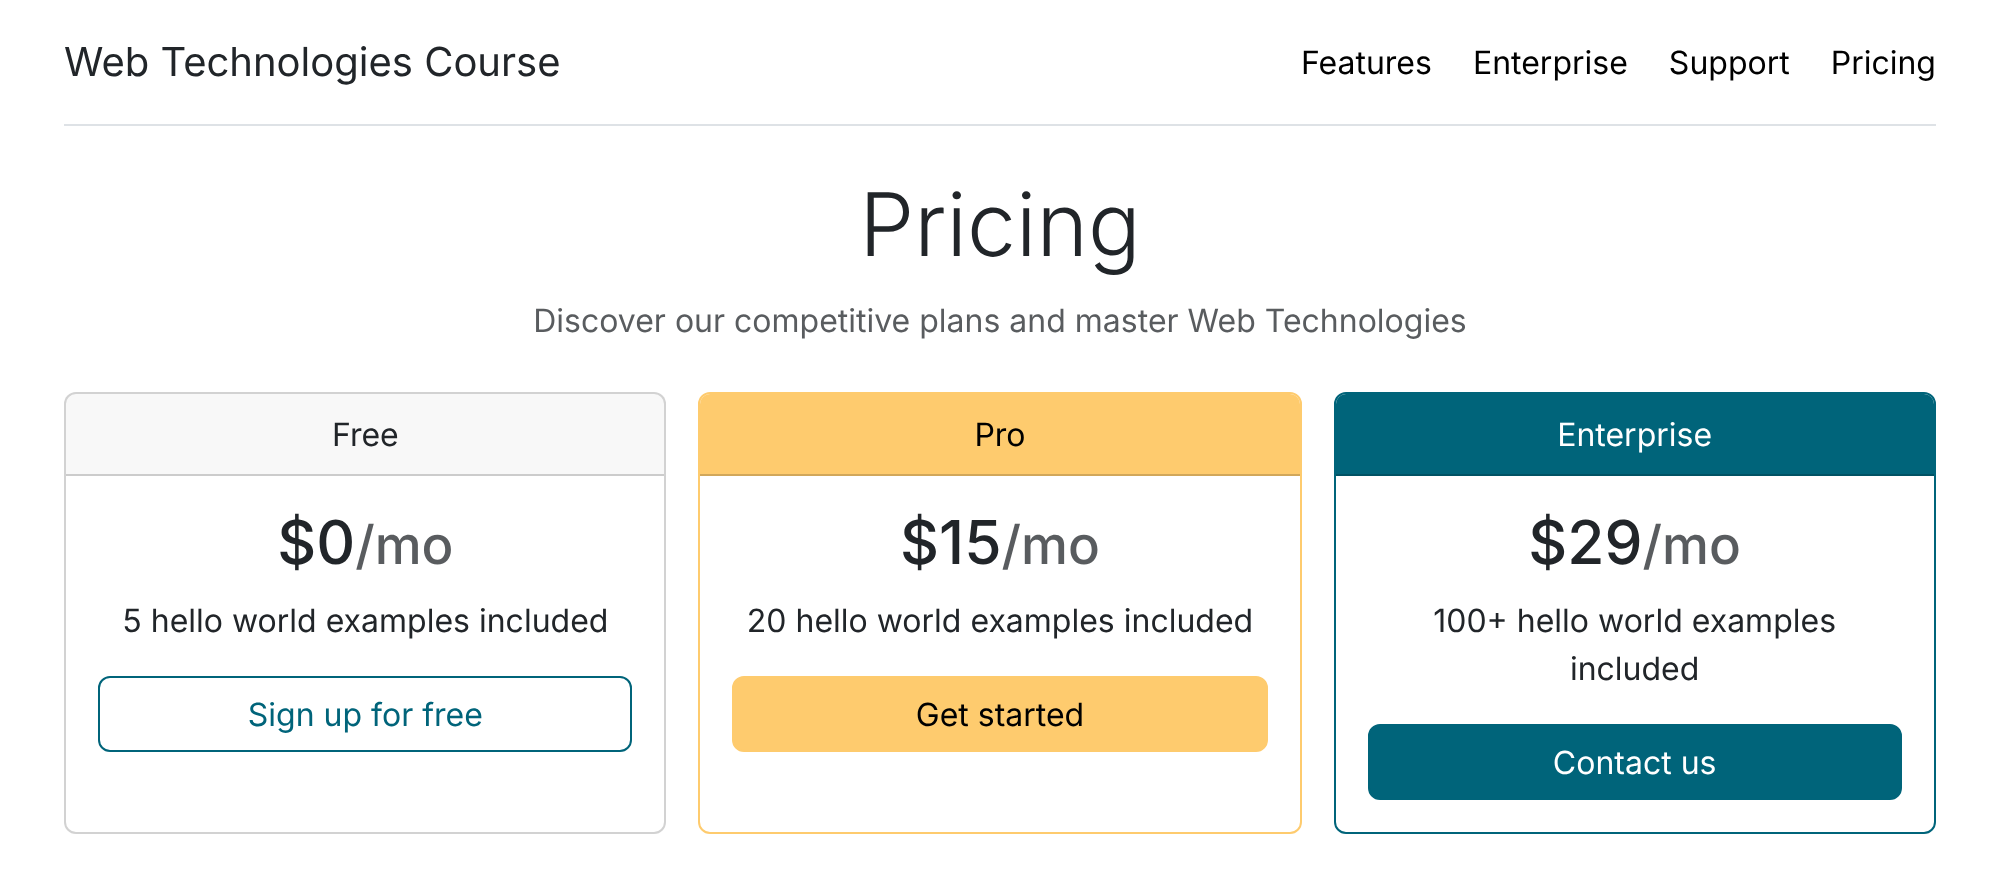
\includegraphics[width=0.92\linewidth]{sources/frontend-bootstrap-custom.png}
\end{browser}

Le classi sono quelle di prima, i colori quelli scelti da noi. Si noti un
dettaglio: sul giallo chiaro di \code{\$secondary} Bootstrap ha scritto il testo
in nero, non in bianco. Il framework sceglie da sé il colore del testo con un
contrasto sufficiente rispetto allo sfondo: è il vantaggio di ricompilare il
framework anziché sovrascriverne i colori a mano.

\section{Bundling e minificazione}

\subsection{Bundling}

\dfn{Bundling}{
  Il \term{bundling} combina più file CSS o JavaScript in un unico file, così
  che il browser effettui \textbf{meno richieste HTTP} per caricare una
  pagina.}

Le richieste HTTP aggiuntive introducono latenza. Le strategie di caching
aiutano nei caricamenti successivi, ma includere molti fogli di stile e molti
script ha comunque un impatto sul \textbf{primo} caricamento: il bundling è
un'ottimizzazione ampiamente adottata.

\begin{affianco}[0.5]
\begin{lstlisting}[style=html, name=prima.html]
<link rel="stylesheet" href="a.css">
<link rel="stylesheet" href="b.css">
<!-- altri fogli di stile -->
<script src="a.js"></script>
<script src="b.js"></script>
<script src="c.js"></script>
<!-- altri script -->
\end{lstlisting}
\risultato
\begin{lstlisting}[style=html, name=dopo.html]
<link rel="stylesheet" href="bundle.css">
<script src="bundle.js"></script>
\end{lstlisting}
\end{affianco}

\warning{L'ordine conta}{
  L'ordine in cui i singoli file vengono accodati nel bundle è significativo: per
  il CSS decide chi vince nella cascata a parità di specificità, per JavaScript
  decide quali definizioni sono disponibili al momento dell'esecuzione.}

\begin{warningbox}{{Uno script che il browser non esegue}}
  Nelle slide gli script sono inclusi con l'attributo
  \code{type="javascript"}. Ma \code{javascript} non è un tipo valido per l'attributo
  \attr{type}: i valori riconosciuti sono un tipo MIME JavaScript, come
  \code{text/javascript}, oppure \code{module}. Con qualunque altro valore il
  browser considera il contenuto un blocco di dati e \textbf{non lo esegue}. Lo
  verifichiamo con Chromium: ogni script imposta una variabile, e lo script di
  prova controlla quali sono state impostate.

  \begin{console}[Terminale]
$ node script.js
type="javascript"      -> ignorato
type="text/javascript" -> eseguito
senza type             -> eseguito
\end{console}

  Per gli script classici l'attributo si omette, come nei listati qui sopra.
  (Nella seconda slide manca anche il tag di chiusura \tg{/script}.)
\end{warningbox}

\info{Una nota storica}{
  Prima che i moduli ES fossero disponibili nei browser (capitolo 6) non
  esisteva alcun modo di scrivere codice JavaScript modulare lato client.
  Strumenti come \term{Webpack}, \term{Rollup} e \term{Parcel} nacquero proprio
  per concatenare tutti i moduli sorgente in una forma che i browser potessero
  comprendere.}

Vediamo un bundler all'opera: \term{esbuild}, uno dei più veloci. Il nostro
programma ha due moduli di funzioni e un punto di ingresso che ne usa una per
modulo:

\begin{affianco}[0.5]
\begin{lstlisting}[style=js, name=src/matematica.js]
export function somma(a, b) {
  return a + b;
}

export function prodotto(a, b) {
  return a * b;
}

export function potenza(base, esponente) {
  return base ** esponente;
}
\end{lstlisting}
\risultato
\begin{lstlisting}[style=js, name=src/stringhe.js]
export function maiuscolo(s) {
  return s.toUpperCase();
}

export function inverti(s) {
  return [...s].reverse().join('');
}
\end{lstlisting}
\begin{lstlisting}[style=js, name=src/index.js]
import { somma } from './matematica.js';
import { maiuscolo } from './stringhe.js';

console.log(maiuscolo('risultato: ') + somma(2, 3));
\end{lstlisting}
\end{affianco}

Con \code{-{}-bundle}, esbuild parte dal punto di ingresso, segue gli
\code{import} e mette tutto in un unico file. Per vedere il bundle
\guillemotleft grezzo\guillemotright\ disattiviamo per un momento il tree shaking,
di cui parliamo subito dopo:

\begin{console}[Terminale]
$ npx esbuild src/index.js --bundle --format=esm --tree-shaking=false
// src/matematica.js
function somma(a, b) {
  return a + b;
}
function prodotto(a, b) {
  return a * b;
}
function potenza(base, esponente) {
  return base ** esponente;
}

// src/stringhe.js
function maiuscolo(s) {
  return s.toUpperCase();
}
function inverti(s) {
  return [...s].reverse().join("");
}

// src/index.js
console.log(maiuscolo("risultato: ") + somma(2, 3));
\end{console}

Gli \code{import} e gli \code{export} sono spariti: i moduli sono stati
concatenati nell'ordine giusto, ciascuno preceduto da un commento con il file di
origine, e il risultato funziona anche in un browser che dei moduli non sa nulla.

\subsection{Tree shaking}

I \textit{bundler} eseguono spesso anche il \term{tree shaking}, cioè
l'eliminazione del codice morto (letteralmente, \guillemotleft scuotere
l'albero\guillemotright\ perché ne cadano le foglie secche).

Spesso ci serve solo una parte delle funzionalità dei moduli che importiamo, e i
moduli possono essere piuttosto grandi: includere un intero modulo nel codice
distribuito con le nostre pagine quando ne usiamo una sola funzione è
inefficiente. Il tree shaking analizza importazioni ed esportazioni per
\textbf{potare} dal bundle finale tutto il codice inutilizzato, con un impatto
notevole sulla dimensione del bundle e quindi sulle prestazioni di caricamento.

\begin{figure}[H]
  \centering
  \begin{tikzpicture}[font=\Lato\scriptsize,
      ent/.style={rounded corners=3pt, fill=primary!70!black, text=white,
                  minimum width=1.5cm, minimum height=0.5cm, font=\FiraCodeNL\scriptsize},
      mod/.style={ellipse, draw=primary!60!black, fill=primary!12!white, line width=0.7pt,
                  minimum width=1.6cm, minimum height=0.6cm, inner sep=1pt},
      fil/.style={circle, draw=primary!60!black, fill=primary!8!white, line width=0.6pt,
                  minimum size=0.62cm, inner sep=0pt, align=center, font=\Lato\tiny},
      fun/.style={rectangle, draw=primary!50!black, fill=white, line width=0.5pt,
                  minimum width=0.82cm, minimum height=0.34cm, inner sep=1pt, font=\Lato\tiny},
      morto/.style={draw=red-gradient-5, fill=red-gradient-1!35!white, dashed,
                    text=red-gradient-6!80!black},
      a/.style={-{Stealth[length=3.5pt,width=3pt]}, line width=0.6pt,
                draw=neutral!45!black},
      am/.style={a, dashed, draw=red-gradient-5}]

    \node[ent] (i) at (5.8,0) {index.js};
    \node[mod] (ma) at (1.35,1.2) {Modulo A};
    \node[mod] (mb) at (5.8,1.2) {Modulo B};
    \node[mod] (mc) at (10.8,1.2) {Modulo C};
    \foreach \m in {ma, mb, mc} \draw[a] (i) -- (\m);

    % file: numero/x/stato (v = usato, m = mai usato)/modulo di appartenenza
    \foreach \n/\x/\st/\m in {1/0.3/m/ma, 2/1.35/v/ma, 3/2.4/v/ma,
                             4/4.0/m/mb, 5/5.1/m/mb, 6/6.3/v/mb, 7/7.6/v/mb,
                             8/10.8/v/mc} {
      \if\st m
        \node[fil, morto] (f\n) at (\x,2.6) {File\\\n};
        \draw[am] (\m) -- (f\n);
      \else
        \node[fil] (f\n) at (\x,2.6) {File\\\n};
        \draw[a] (\m) -- (f\n);
      \fi
    }

    % funzioni: file di appartenenza/x/stato
    \foreach \f/\x/\st in {1/0.3/m, 2/1.35/v, 3/2.4/v, 4/3.6/m, 4/4.5/m,
                           5/5.4/m, 6/6.3/m, 6/7.2/v, 7/8.1/v, 7/9.0/v,
                           8/9.95/v, 8/10.8/v, 8/11.65/v} {
      \if\st m
        \node[fun, morto] (g) at (\x,3.55) {function};
        \draw[am] (f\f) -- (g);
      \else
        \node[fun] (g) at (\x,3.55) {function};
        \draw[a] (f\f) -- (g);
      \fi
    }

    \node[font=\Lato\scriptsize, text=red-gradient-6!80!black, anchor=west, align=left]
      at (7.9,-0.35) {in rosso: codice mai usato,\\escluso dal bundle};
  \end{tikzpicture}
  \caption{Il tree shaking: \texttt{index.js} importa tre moduli, ma dal
           bundle restano solo i file e le funzioni effettivamente
           raggiungibili.}
  \label{fig:tree-shaking}
\end{figure}

È quello che esbuild fa da sé, quando non lo disattiviamo:

\begin{console}[Terminale]
$ npx esbuild src/index.js --bundle --format=esm
// src/matematica.js
function somma(a, b) {
  return a + b;
}

// src/stringhe.js
function maiuscolo(s) {
  return s.toUpperCase();
}

// src/index.js
console.log(maiuscolo("risultato: ") + somma(2, 3));
\end{console}

Di cinque funzioni ne restano due, le sole che \code{index.js} usa. Il tree
shaking funziona bene con i moduli ES perché \code{import} ed \code{export} sono
\textbf{statici}: si possono analizzare senza eseguire il programma.

\subsection{Minificazione}

Quando scriviamo codice, l'indentazione e i nomi significativi delle variabili
sono essenziali per leggibilità, comprensibilità e manutenibilità. Ai browser,
però, non serve codice leggibile: possiamo ottimizzare il trasferimento
rimuovendo gli spazi \guillemotleft superflui\guillemotright\ e accorciando il
codice senza alterarne il funzionamento. È la \term{minificazione}, e i file
risultanti si dicono \textbf{minificati}. Proviamo con \term{Terser}, uno dei
minificatori più usati, sull'esempio delle slide:

\begin{lstlisting}[style=js, name=msg.js]
let msg = "Hello";
let name = "Web Technologies";
let str = `${msg}, ${name}!`;
let b = true;
if(b === true)
  document.getElementById('msg').innerHTML = str;
\end{lstlisting}

\begin{console}[Terminale]
$ wc -c msg.js
159 msg.js
$ npx terser msg.js --compress --mangle
let msg="Hello",name="Web Technologies",str=`${msg}, ${name}!`,b=!0;!0===b&&(document.getElementById("msg").innerHTML=str);
$ npx terser msg.js --compress --mangle -o msg.min.js
$ wc -c msg.min.js
123 msg.min.js
\end{console}

Le dichiarazioni sono state fuse in una sola, \code{true} è diventato
\code{!0} (due caratteri invece di quattro, stesso valore) e l'\code{if} un
\code{\&\&}, che valuta il secondo operando solo se il primo è vero. Il file
minificato pesa 123 byte, come nelle slide. Due differenze, però:

\begin{itemize}
  \item nelle slide il file originale pesa 188 byte, e il risparmio sale al
        34,57\%; il nostro, con le stesse righe, ne pesa 159, e il risparmio è
        di 36 byte, il 22,6\%;
  \item nel codice minificato delle slide manca lo spazio dentro il template
        literal: \code{`\$\{msg\},\$\{name\}!`}. Un minificatore non lo
        toglierebbe mai, perché fa parte della \textbf{stringa}: la pagina
        mostrerebbe \guillemotleft Hello,Web Technologies!\guillemotright. E
        infatti i 123 byte tornano proprio contando lo spazio.
\end{itemize}

Terser non ha accorciato i nomi delle variabili: sono dichiarate al livello più
esterno di uno script classico, quindi \textbf{globali}, e altri script della
pagina potrebbero usarle. Se gli diciamo che non è così (\code{-{}-toplevel}),
il minificatore si spinge molto più in là:

\begin{console}[Terminale]
$ npx terser msg.js --compress --mangle --toplevel
document.getElementById("msg").innerHTML="Hello, Web Technologies!";
\end{console}

Ha calcolato in anticipo il valore della stringa e ha eliminato tutte le
variabili. È corretto solo se nessun altro script le usa: per questo
l'opzione va chiesta esplicitamente (i bundler, che conoscono tutto il codice
dell'applicazione, possono permettersela).

L'effetto della minificazione è tanto maggiore quanto più grandi sono i file
sorgente. Le slide citano React 18.2.0 (circa 85\,kB, che minificato scende a
circa 25\,kB, il 70\% in meno) e Moment.js 2.29.4 (circa 151\,kB, che scende a
circa 75\,kB, il 50\% in meno). Rifacciamo le misure sui pacchetti npm:

\begin{console}[Terminale]
$ npm pack react@18.2.0 moment@2.29.4 --silent
react-18.2.0.tgz
moment-2.29.4.tgz
$ tar -xzf react-18.2.0.tgz && mv package react
$ tar -xzf moment-2.29.4.tgz && mv package moment
$ wc -c react/cjs/react.development.js moment/dist/moment.js
 87574 react/cjs/react.development.js
154671 moment/dist/moment.js
242245 total
$ npx terser react/cjs/react.development.js --compress --mangle | wc -c
26255
$ npx terser moment/dist/moment.js --module | wc -c
96339
$ npx terser moment/dist/moment.js --module --compress | wc -c
88179
$ npx terser moment/dist/moment.js --module --mangle | wc -c
63074
$ npx terser moment/dist/moment.js --module --compress --mangle | wc -c
59072
\end{console}

Per React i conti tornano: 87\,574 byte sono 85,5\,KiB, e minificati con Terser
diventano 25,6\,KiB, il 70\% in meno. Per Moment.js i 151\,KiB tornano, ma
Terser fa meglio dei 75\,kB delle slide: 57,7\,KiB, il 62\% in meno. Le quattro
misure su Moment.js mostrano da dove viene il risparmio:

\begin{center}
\renewcommand{\arraystretch}{1.35}
\begin{tabular}{@{}l@{\hspace{1cm}}r@{\hspace{1cm}}r@{}}
  \textbf{Opzioni di Terser} & \textbf{Byte} & \textbf{Risparmio} \\
  nessuna: via spazi e commenti   &  96\,339 & 38\% \\
  \code{-{}-compress}               &  88\,179 & 43\% \\
  \code{-{}-mangle}                 &  63\,074 & 59\% \\
  \code{-{}-compress -{}-mangle}    &  59\,072 & 62\% \\
\end{tabular}
\end{center}

Il guadagno più grande viene dal \textit{mangling}, cioè dal rinominare con una
lettera le variabili locali e i parametri; \code{-{}-compress} riscrive le
espressioni in forme più brevi, come abbiamo visto. Il risultato dipende quindi
dallo strumento e dalle opzioni, e i numeri delle slide vanno letti come ordini
di grandezza.

\info{Minificazione e compressione}{
  La minificazione non sostituisce la compressione che i server applicano alle
  risposte (gzip o Brotli, segnalata dall'header \code{Content-Encoding}): le
  due si sommano. Il file \code{moment.js} ufficiale pesa 174\,604 byte, che
  compressi con gzip diventano 36\,720; la versione minificata
  \code{min/moment.min.js} ne pesa 58\,103, e compressa 18\,553. Per questo Vite,
  come vedremo, riporta per ogni file anche la dimensione dopo gzip.}

Anche il CSS si minifica, ma con risultati più modesti: non ci sono variabili da
rinominare, solo spazi, commenti e qualche abbreviazione. Il CSS di Bootstrap
passa da 280\,620 a 232\,360 byte, il 17\% in meno; la nostra versione
personalizzata, compilata da Sass con \code{-{}-style=compressed}, è dello
stesso ordine:

\begin{console}[Terminale]
$ sass --load-path=node_modules --quiet-deps --silence-deprecation=import --style=compressed --no-source-map scss/custom2.scss css/custom.min.css
$ ls -l css/custom.min.css node_modules/bootstrap/dist/css/bootstrap.css node_modules/bootstrap/dist/css/bootstrap.min.css
-rw-r--r-- 1 root root 233617 Nov 20 09:14 css/custom.min.css
-rw-r--r-- 1 root root 280620 Nov 20 09:13 node_modules/bootstrap/dist/css/bootstrap.css
-rw-r--r-- 1 root root 232360 Nov 20 09:13 node_modules/bootstrap/dist/css/bootstrap.min.css
\end{console}

Bundling, tree shaking e minificazione, di solito, si fanno insieme. Ecco il
nostro piccolo programma, impacchettato, potato e minificato da esbuild in una
sola riga, ed eseguito:

\begin{console}[Terminale]
$ npx esbuild src/index.js --bundle --format=esm --minify --outfile=dist/bundle.js --log-level=warning
$ cat dist/bundle.js
function r(o,n){return o+n}function t(o){return o.toUpperCase()}console.log(t("risultato: ")+r(2,3));
$ node dist/bundle.js
RISULTATO: 5
\end{console}

Nel bundle minificato \code{somma} e \code{maiuscolo} si chiamano \code{r} e
\code{t}: in un bundle i nomi non sono più globali, e il minificatore li può
accorciare. Strumenti come Vite fanno tutto questo in automatico.

\section{Vite}

\term{Vite} (si pronuncia \guillemotleft vit\guillemotright, come la parola
francese che significa \guillemotleft rapido\guillemotright) è uno strumento che
assiste lo sviluppatore sia durante lo sviluppo sia al momento del rilascio. Ha
due componenti chiave:

\begin{itemize}
  \item un \textbf{server di sviluppo} con numerose funzionalità avanzate per
        snellire il lavoro;
  \item uno \textbf{strumento di build} per creare risorse statiche altamente
        ottimizzate, pronte per la produzione.
\end{itemize}

Sotto il cofano Vite riunisce strumenti del tipo visto finora: Vite 8 usa
\term{Rolldown}, un bundler scritto in Rust, e \term{Lightning CSS} per
minificare il CSS; e se nel progetto c'è una configurazione di PostCSS, la
applica da sé a tutto il CSS importato.

\subsection{Creare un progetto}

Si parte con \code{npm create vite@latest}, che scarica ed esegue lo strumento
di inizializzazione \code{create-vite}. In un terminale interattivo il comando
pone le domande della slide: il nome del progetto, il framework (Vanilla, cioè
nessuno, Vue, React, Preact, Lit, Svelte, Solid, Qwik\ldots) e la variante
(TypeScript o JavaScript). Le stesse risposte si possono dare sulla riga di
comando (le opzioni dopo \code{-{}-} vanno a \code{create-vite}, non a npm):

{\wtglifi
\begin{console}[Terminale]
$ npm create vite@latest hello-vite -- --template vanilla-ts --no-interactive

> npx
> cva hello-vite --template vanilla-ts --no-interactive


create-vite v9.3.4

|
o  Scaffolding project in [cartella del progetto]...
|
¯  Done. Now run:

  cd hello-vite
  npm install
  npm run dev
\end{console}
}

Il modello \code{vanilla-ts} usa TypeScript senza framework. Ecco lo scheletro
generato:

\begin{affianco}[0.42]
\begin{console}[Terminale]
$ find . -type f | sort
./.gitignore
./index.html
./package.json
./public/favicon.svg
./public/icons.svg
./src/assets/hero.png
./src/assets/typescript.svg
./src/assets/vite.svg
./src/counter.ts
./src/main.ts
./src/style.css
./tsconfig.json
\end{console}
\risultato
\begin{lstlisting}[style=json, name=package.json]
{
  "name": "hello-vite",
  "private": true,
  "version": "0.0.0",
  "type": "module",
  "scripts": {
    "dev": "vite",
    "build": "tsc && vite build",
    "preview": "vite preview"
  },
  "devDependencies": {
    "typescript": "~7.0.2",
    "vite": "^8.3.6"
  }
}
\end{lstlisting}
\end{affianco}

Le dipendenze sono solo di sviluppo: Vite e TypeScript servono a costruire
l'applicazione, non a eseguirla (nelle slide le versioni sono TypeScript 6 e
Vite 8.0, e il progetto si chiama \code{vite-new} invece di \code{hello-vite}).
I tre script sono il cuore del flusso di lavoro:

\begin{center}
\renewcommand{\arraystretch}{1.4}
\begin{tabular}{@{}l@{\hspace{1.2cm}}>{\raggedright\arraybackslash}p{8.8cm}@{}}
  \textbf{Comando} & \textbf{Effetto} \\
  \code{dev}     & avvia il server di sviluppo. Vite osserva le modifiche ai
                   file sorgente e aggiorna automaticamente l'applicazione
                   (\textit{live reload}). \\
  \code{build}   & genera un bundle ottimizzato, pronto per la produzione. \\
  \code{preview} & è un semplice server statico che serve i file generati
                   durante la fase di build. \\
\end{tabular}
\end{center}

\subsection{Il server di sviluppo}

Installiamo le dipendenze e avviamo il server:

{\wtglifi
\begin{console}[Terminale]
$ npm install

added 17 packages, and audited 18 packages in 2s

8 packages are looking for funding
  run `npm fund` for details

found 0 vulnerabilities
$ npm run dev

> hello-vite@0.0.0 dev
> vite


  VITE v8.3.8  ready in 147 ms

  ¤  Local:   http://localhost:5173/
  ¤  Network: use --host to expose
\end{console}
}

Nelle slide il server di sviluppo è un Vite 6.3.5, mentre la build più avanti è
di Vite 8.0.10: le due schermate vengono da momenti diversi. Il server ascolta
solo sull'interfaccia locale; per raggiungerlo da un altro dispositivo, per
esempio un telefono sulla stessa rete, si aggiunge l'opzione \code{-{}-host}.
Ecco la pagina del modello:

\begin{browser}[localhost:5173]
  \centering
\includegraphics[width=0.8\linewidth]{sources/frontend-vite.png}
\end{browser}

Il server è pronto in poco più di un decimo di secondo perché, in sviluppo,
Vite \textbf{non impacchetta} il codice dell'applicazione. Il browser carica i file sorgente come
moduli ES (capitolo 6), uno per uno, e Vite trasforma al volo ogni file nel
momento in cui viene richiesto. Chiediamo a mano \code{counter.ts}:

\begin{console}[Terminale]
$ curl -s http://localhost:5173/src/counter.ts | head -n 9
export function setupCounter(element) {
    let counter = 0;
    const setCounter = (count) => {
        counter = count;
        element.innerHTML = `Count is ${counter}`;
    };
    element.addEventListener("click", () => setCounter(counter + 1));
    setCounter(0);
}
\end{console}

È già JavaScript: le annotazioni di tipo (\code{element: HTMLButtonElement},
\code{count: number}) sono state tolte, senza controllarle, come fa il
\textit{type stripping} di Node visto nel capitolo 19. Il controllo dei tipi
resta compito di \code{tsc}.

Quando salviamo un file, Vite non si limita a ricaricare la pagina: attraverso
una connessione WebSocket le invia il solo modulo modificato, che viene
sostituito \guillemotleft a caldo\guillemotright, senza perdere lo stato
dell'applicazione quando è possibile. È la \term{Hot Module Replacement}
(HMR), quella che la pagina del modello invita a provare.

\subsection{Aggiungere Sass}

Supponiamo di voler aggiungere un foglio di stile Sass. Prima di tutto
installiamo \code{sass} fra le dipendenze di sviluppo del progetto:

\begin{console}[Terminale]
$ npm install -D sass

added 11 packages, and audited 29 packages in 723ms

13 packages are looking for funding
  run `npm fund` for details

found 0 vulnerabilities
\end{console}

Nella slide l'opzione è scritta \code{–D}, con un trattino tipografico al posto
del trattino normale (come il \code{–target} del capitolo 19). Copiato nel
terminale, il comando fallisce, e npm ha anche la cortesia di spiegare perché:

{\wtglifi
\begin{console}[Terminale]
$ npm install ¬D sass
npm error arg Argument starts with non-ascii dash, this is probably invalid: ¬D
npm error code EINVALIDTAGNAME
npm error Invalid tag name "¬D" of package "¬D": Tags may not have any characters that encodeURIComponent encodes.
...
\end{console}
}

Poi creiamo il foglio di stile, con una variabile, una regola annidata e una
funzione del modulo \code{sass:color}:

\begin{lstlisting}[style=css, name=src/custom.scss]
@use "sass:color";

$arancione: #f28c28;

#center h1 {
  color: $arancione;
}

.counter {
  color: white;
  background: $arancione;

  &:hover {
    border-color: color.adjust($arancione, $lightness: -15%);
  }
}
\end{lstlisting}

Infine diciamo a Vite che il file fa parte dell'applicazione, importandolo in
\code{main.ts} (riga 2), e già che ci siamo cambiamo il titolo (riga 16):

\begin{lstlisting}[style=ts, name=src/main.ts]
import './style.css'
import './custom.scss'
import heroImg from './assets/hero.png'
import typescriptLogo from './assets/typescript.svg'
import viteLogo from './assets/vite.svg'
import { setupCounter } from './counter.ts'
\end{lstlisting}

\begin{lstlisting}[style=ts, name=src/main.ts, firstnumber=15]
  <div>
    <h1>Hello Web Technologies!</h1>
    <p>Edit <code>src/main.ts</code> and save to test <code>HMR</code></p>
  </div>
\end{lstlisting}

Vite riconosce dall'estensione che si tratta di un file Sass, lo compila con il
pacchetto \code{sass} e lo accoda al CSS originale. Il nuovo stile vince perché
arriva dopo, a parità di specificità (\code{.counter}), o perché è più
specifico (\code{\#center h1}):

\begin{browser}[localhost:5173]
  \centering
\includegraphics[width=0.8\linewidth]{sources/frontend-vite-sass.png}
\end{browser}

Come arriva al browser un file Sass? Anche lui diventa un modulo JavaScript:

\begin{console}[Terminale]
$ curl -s http://localhost:5173/src/custom.scss | head -n 4
import { createHotContext as __vite__createHotContext } from "/@vite/client";import.meta.hot = __vite__createHotContext("/src/custom.scss");import { updateStyle as __vite__updateStyle, removeStyle as __vite__removeStyle } from "/@vite/client"
const __vite__id = "[cartella del progetto]/src/custom.scss"
const __vite__css = "#center h1 {\n  color: #f28c28;\n}\n\n.counter {\n  color: white;\n  background: #f28c28;\n}\n.counter:hover {\n  border-color: rgb(75.9932920537%, 39.9406604747%, 4.5949432405%);\n}"
__vite__updateStyle(__vite__id, __vite__css)
\end{console}

Il CSS compilato da Sass è una stringa (\code{\_\_vite\_\_css}), che la funzione
\code{\_\_vite\_\_updateStyle} inserisce nella pagina in un elemento
\tg{style}. Quando il file cambia, Vite sostituisce solo questo modulo, e la
pagina cambia aspetto senza ricaricarsi.

\subsection{La build}

Quando l'applicazione è pronta, si costruisce la versione di produzione:

{\wtglifi
\begin{console}[Terminale]
$ npm run build

> hello-vite@0.0.0 build
> tsc && vite build

vite v8.3.8 building client environment for production...
transforming...
¢ 10 modules transformed.
rendering chunks...
computing gzip size...
dist/index.html                  0.45 kB ¦ gzip: 0.29 kB
dist/assets/vite-BF8QNONU.svg    8.70 kB ¦ gzip: 1.60 kB
dist/assets/hero-CLDdwZDr.png   13.05 kB
dist/assets/index-be7Yw0bP.css   4.20 kB ¦ gzip: 1.49 kB
dist/assets/index-Dqtoo5RJ.js    4.50 kB ¦ gzip: 2.03 kB

¢ built in 205ms
\end{console}
}

Lo script esegue prima \code{tsc}, che \textbf{controlla} i tipi senza produrre
file (nel \code{tsconfig.json} del modello c'è \code{"noEmit": true}); grazie a
\code{\&\&}, \code{vite build} parte solo se il controllo è andato a buon fine.
In questa fase Vite ha fatto molto lavoro per noi:

\begin{itemize}
  \item ha analizzato quali risorse statiche l'applicazione usa davvero (le
        immagini importate in \code{main.ts}; il logo di TypeScript è finito
        dentro il JavaScript, perché i file piccoli vengono incorporati);
  \item ha compilato il file Sass in CSS e quelli TypeScript in JavaScript;
  \item ha riunito il CSS originale e quello di Sass in un unico file, e i file
        JavaScript in un altro;
  \item ha minificato i bundle;
  \item ha applicato il \term{fingerprinting} ai nomi dei file finali;
  \item ha spostato tutto nella cartella \code{dist}, aggiornando
        \code{index.html} con i riferimenti corretti ai bundle.
\end{itemize}

\begin{affianco}[0.4]
\begin{console}[Terminale]
$ find dist -type f | sort
dist/assets/hero-CLDdwZDr.png
dist/assets/index-Dqtoo5RJ.js
dist/assets/index-be7Yw0bP.css
dist/assets/vite-BF8QNONU.svg
dist/favicon.svg
dist/icons.svg
dist/index.html
\end{console}
\risultato
\begin{lstlisting}[style=html, name=dist/index.html]
<!doctype html>
<html lang="en">
  <head>
    <meta charset="UTF-8" />
    <link rel="icon" type="image/svg+xml" href="/favicon.svg" />
    <meta name="viewport" content="width=device-width, initial-scale=1.0" />
    <title>hello-vite</title>
    <script type="module" crossorigin src="/assets/index-Dqtoo5RJ.js"></script>
    <link rel="stylesheet" crossorigin href="/assets/index-be7Yw0bP.css">
  </head>
  <body>
    <div id="app"></div>
  </body>
</html>
\end{lstlisting}
\end{affianco}

I file della cartella \code{public} (\code{favicon.svg}, \code{icons.svg}) sono
copiati così come sono, con il loro nome. Il bundle JavaScript, minificato,
comincia così:

\begin{console}[Terminale]
$ head -c 200 dist/assets/index-*.js
(function(){let e=document.createElement(`link`).relList;if(e&&e.supports&&e.supports(`modulepreload`))return;for(let e of document.querySelectorAll(`link[rel="modulepreload"]`))n(e);new MutationObser
\end{console}

\subsection{Fingerprinting dei nomi}

I bundle prodotti hanno nomi curiosi: \code{index-be7Yw0bP.css},
\code{index-Dqtoo5RJ.js}. L'ultima parte del nome è un \textbf{hash} del
contenuto: costruendo una nuova versione dell'applicazione, se i file cambiano,
cambia anche il nome. E se il contenuto è lo stesso, il nome è lo stesso:
\code{vite-BF8QNONU.svg} e \code{hero-CLDdwZDr.png} sono identici a quelli delle
slide, prodotti su un altro computer, con un'altra versione di Vite, perché le
immagini del modello sono le stesse. Il CSS e il JavaScript invece hanno nomi
diversi, perché il loro contenuto è diverso (c'è il nostro file Sass, e il
modello è cambiato).

Mettiamolo alla prova. Calcoliamo l'impronta MD5 dei due bundle, cambiamo
\textbf{solo} il colore nel file Sass, ricostruiamo e ricalcoliamo:

\begin{console}[Terminale]
$ md5sum dist/assets/index-*
b5526340394007fe0ddabe2af5a8f072  dist/assets/index-Dqtoo5RJ.js
692b94661365352ff9a79b733a21aeaa  dist/assets/index-be7Yw0bP.css
$ sed -i 's/#f28c28/#2a9d8f/' src/custom.scss
$ npm run build > /dev/null
$ md5sum dist/assets/index-*
1f4c983ea2adf3534ee56e86ec27bdb2  dist/assets/index-CVlKSMY-.css
b5526340394007fe0ddabe2af5a8f072  dist/assets/index-E_qvTPJm.js
\end{console}

Il CSS è cambiato, e ha cambiato nome. Il JavaScript ha cambiato nome anche se
il suo contenuto è identico byte per byte (stessa impronta MD5): l'hash di un
bundle, in Vite, tiene conto anche dei moduli che importa, compreso il CSS. Se
torniamo al colore di prima, tornano i nomi di prima:

\begin{console}[Terminale]
$ sed -i 's/#2a9d8f/#f28c28/' src/custom.scss
$ npm run build > /dev/null
$ ls dist/assets
hero-CLDdwZDr.png
index-Dqtoo5RJ.js
index-be7Yw0bP.css
vite-BF8QNONU.svg
\end{console}

\info{Perché serve}{
  Supponiamo che i file si chiamassero semplicemente \code{index.css} e
  \code{index.js}. Un browser che visita la pagina un minuto prima del rilascio
  di una nuova versione potrebbe continuare a usare per un certo tempo le copie
  vecchie conservate nella propria cache (capitolo 2), e vedere un sito rotto,
  magari con il nuovo HTML e il vecchio CSS. Cambiando il nome a ogni modifica
  il problema scompare: la copia vecchia resta valida, ma nessuno la richiede
  più. Anzi, i file con l'impronta nel nome si possono mettere in cache
  \guillemotleft per sempre\guillemotright\ (per esempio con
  \code{Cache-Control: max-age=31536000, immutable}), mentre \code{index.html},
  che contiene i nomi aggiornati, va ricontrollato a ogni visita.}

\subsection{L'anteprima}

Lo script \code{preview} serve la cartella \code{dist} così com'è, per provare
la build prima di pubblicarla:

{\wtglifi
\begin{console}[Terminale]
$ npm run preview

> hello-vite@0.0.0 preview
> vite preview

  ¤  Local:   http://localhost:4173/
  ¤  Network: use --host to expose
\end{console}
}

È un server di prova, non di produzione: risponde a tutto con
\code{Cache-Control: no-cache}, anche per i file con l'impronta.

\begin{console}[Terminale]
$ curl -sI http://localhost:4173/assets/index-be7Yw0bP.css
HTTP/1.1 200 OK
Vary: Origin
Content-Length: 4204
Content-Type: text/css
Last-Modified: Fri, 20 Nov 2026 09:18:54 GMT
ETag: W/"4204-1795166334790"
Cache-Control: no-cache
Date: Fri, 20 Nov 2026 09:18:55 GMT
Connection: keep-alive
Keep-Alive: timeout=5
\end{console}

In produzione la cartella \code{dist} si pubblica su un qualunque server di file
statici (NGINX, capitolo 10, o un servizio di hosting), configurato con le
intestazioni di cache appropriate.

\section{Riferimenti}

\begin{itemize}
  \item \textbf{Client-side Tooling Overview} --- MDN web docs. \\
        \urlx{https://developer.mozilla.org/en-US/docs/Learn/Tools_and_testing/Understanding_client-side_tools/Overview}
  \item \textbf{Sass: Guide}. \\
        \urlx{https://sass-lang.com/guide/}
  \item \textbf{PostCSS} e \textbf{Browserslist}. \\
        \urlx{https://postcss.org/} \quad \urlx{https://browsersl.ist/}
  \item \textbf{Bootstrap: Getting Started}. \\
        \urlx{https://getbootstrap.com/docs/5.3/getting-started/introduction/}
  \item \textbf{Get started with Tailwind CSS}. \\
        \urlx{https://tailwindcss.com/docs/installation}
  \item \textbf{Terser} ed \textbf{esbuild}. \\
        \urlx{https://terser.org/} \quad \urlx{https://esbuild.github.io/}
  \item \textbf{Vite: Official Guide}. \\
        \urlx{https://vitejs.dev/guide/}
\end{itemize}
